\subsection{Towards stability} \label{subsec_on_stability}

In several disciplines, stability has been defined as \emph{Bounded Input Bounded Output}
(BIBO). It is the fundamental property of a system when subjected to bounded input
disturbances. BIBO stability ensures that the output of a system will also be bounded,
preventing uncontrolled or unexpected behavior \parencite[270]{mannaert_normalized_2016}. 

A real-world example of the importance of stability is the Tacoma Narrows Bridge in
Washington State, USA. This bridge, depicted in Figure \ref*{fig_bridge}, collapsed on
November the 7th, 1940. This was caused due to wind-induced oscillations called
aeroelastic flutter. The wind (Input) induced oscillations in the bridge, causing it to
start swaying back and forth (Output). These oscillations were initially small, but as
they continued, they began to increase in amplitude and magnitude. Eventually, this 
caused the bridge to collapse.

\begin{figure}[H]
    \centering
    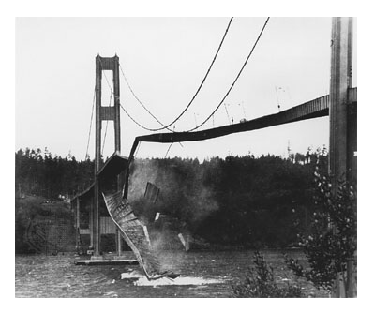
\includegraphics[width=0.6\textwidth]{figures/bridge.pdf}
    \caption[Tacoma Narrows Bridge]{Tacoma Narrows Bridge (Galloping Gertie)}
    \label{fig_bridge}
\end{figure}

Stability can also be used in the context of software engineering. In the context of
\gls{ns}, it is considered a critical property that ensures that the software is not
excessively sensitive to small changes \parencite[270]{mannaert_normalized_2016}. New
functional requirements should only lead to a fixed and expected amount of changes in
the source code. 

Conversely, instabilities occur when the total number of modifications relies on the size
of the software artifact. When there are software instabilities, the number of changes
will grow over time in parallel with the growth of the system. These instabilities are
referred to as combinatorial effects \parencite[270]{mannaert_normalized_2016}. 

When combinatorial effects are absent, the software artifact can be considered evolvable.